%FIXME FIXME FIXME
% talk about auto-detect array size
%FIXME FIXME FIXME

%=====HEADER=====%
\documentclass[a4paper]{article}
\usepackage[utf8]{inputenc}
\usepackage[T1]{fontenc}
\usepackage[english]{babel}
% Pour le petit confort de Ronan Keryell avec Emacs/AUCTeX/Preview-LaTeX:
\usepackage[pdftex,delayed]{preview}
\ifPreview
\else
% Déclenche un bug en mode Preview
\usepackage{hyperref}
\fi
%\usepackage{algorithmic}
%\usepackage{algorithm}
\usepackage[vmargin=3.5cm,hmargin=3.5cm]{geometry}
%\usepackage{amsthm}
%\usepackage{amsmath}
%\usepackage{amssymb}
%\usepackage{mathrsfs}
\usepackage{graphicx}
\usepackage{listings}
%\renewcommand{\algorithmiccomment}[1]{//#1}

\widowpenalty=3000


\newtheorem{defdef}{Definition}

\renewcommand{\lstlistingname}{Source code}
\lstset{
language=c,
numbers=left,
stepnumber=5,
frame=single,
tabsize=4,
captionpos=b
}


%=====TITLE=====%
\title{Generating SMECY API from annotated sequential code with ROSE compiler}
\author{Vincent \sc Lanore}
\date{May to August 2011}

%=====DOCUMENT=====%
\begin{document}
	\maketitle
	
	\begin{abstract}
		During this internship my role was to learn how to use ROSE, a
        compiler infrastructure, and study the possible application to the
        compilation of a set of pragma directives that is part of a
        standard called SME-C defined as part of SMECY European project.
		
		I have implemented a prototype translating annotated C/C++ code to the SME-C low-level API and validated it on a few examples. The present report presents SME-C and ROSE then details the conception and implementation of the prototype.
	\end{abstract}
	
	%\newpage
	\tableofcontents
	\newpage
	
\section*{Introduction}
	This internship took place at HPC Project in Montpellier under the
    direction of Ronan \textsc{Keryell} and Thierry \textsc{Porcher}. It lasted 10 weeks, from May 2011 to August 2011. The original title of the internship was \emph{Generating Par4All Accel from annotated sequential code with ROSE compiler}.
	
	\paragraph{}With the recent stop of CPU frequency increase, multi-core architecture have begun to become more common. Today CPU clusters can count up to hundreds of cores. Moreover, specialized hardware accelerators exist and can speed up greatly some types of computing.  Making the most of these architectures require programs made specifically for them. 
	
	The field is likely to evolve quickly and many already existing programs are fully sequential. Being able to program specialized parallel programs from scratch is one thing but parallelizing existing programs easily could speed up their execution dramatically. Annotation-based methods like OpenMP can easily parallelize a program but work only with shared-memory multi-CPUs architectures.
	
	During this internship I was to work on an ongoing project called SMECY that aims at providing a high-level set of annotations to parallelize code targeting heterogeneous architectures mixing CPUs and hardware accelerators.
	

\section{SME-C}
	This first part presents SME-C and ROSE which are at the heart of the internship. Apart from the work of writing and documentation, nothing here is my own work.
	\subsection{Presenting SME-C}
	\subsubsection{ARTEMIS \& SMECY}
 	\emph{SMECY} stands for \emph{Smart Multicore Embedded
      Systems}.\footnote{\url{http://www.smecy.eu}} SMECY is a European
    project, part of the \emph{ARTEMIS} European project initiative, which stands for \emph{Advanced Research \& Technology for EMbedded Intelligence and Systems}.\footnote{\url{http://www.artemis.eu}} ARTEMIS is a European initiative aiming at rivaling initiatives from Asia and North America in the domain of embedded systems.

	Within ARTEMIS, SMECY focuses on heterogeneous multicore architectures and aims at providing new programming technologies to exploit the potential of such architectures. Targeted architectures may include various hardware accelerators (GPU, FGPA, specialized vector processors\ldots).

	\subsubsection{SME-C}
	SMECY requires a portable intermediate representation to be used
    between programming tools. To increase portability and readability, it
    is based on a programming language and this language is called
    \emph{SME-C}.

	\begin{defdef} In C, a \emph{pragma directive}, often called a \emph{pragma}, is a compiler directive that provides additional information to the compiler.
	\end{defdef}
	
	SME-C adds a few \emph{pragma directives} and an \emph{API} to the C99 language. Indeed, the C language is both portable and expressive while still readable.
	
	The SMECY API is a low-level API that is used to call hardware
    accelerators in a portable way. The SMECY pragma directives are more
    high-level and can be used for parallel execution, mapping to hardware
    or streaming. The complete list of the SMECY API functions is in
    appendix \ref{api}.

	SME-C is designed to work with \emph{OpenMP}, a programming model for shared-memory platforms. SME-C provides directives and API for mapping and streaming while OpenMP provides directives and API for parallelization and synchronization.
	
	\subsubsection{Par4All}
	\emph{Par4All} is an automatic parallelizing and optimizing compiler
    developed notably by HPC Project. Par4All uses a set of macros and API
    functions collectively called \emph{Par4All Accel runtime} to ease
    parallelized code generation by masking implementation-dependent or
    hardware-dependent details. Par4All can parallelize to several CPUs
    (using OpenMP) or GPUs (Cuda, OpenCL).

	Adding the possibilities offered by SME-C to Par4All would extend the Par4All targets with the different architectures that will be supported by SME-C in the future. The work to be done during the internship would go toward such an addition and is destined to be incorporated to Par4All at some point in the future.
	
	\subsection{Toward a SMECY compiler}
	Since SMECY is an ongoing project, there is no implementation of a SME-C compiler yet. In this internship I have worked toward implementing one.
	
	Building a compiler from scratch is a huge task that goes far beyond the scope of the internship. Fortunately, there are ways to use existing front-ends, back-ends or whole compiler infrastructure so as to make the task easier.

	\subsubsection{Source-to-source compiling}
	Since SME-C includes OpenMP, the final compiler needs to compile both SME-C pragmas and API as well as OpenMP pragmas and API.
	
	As many existing compilers already compile OpenMP, it would be interesting to use them. Moreover, mapping and streaming can be done using only a few API functions. This suggests dividing the compilation in two separate parts: first, transforming the input code (that contains SME-C pragmas) into a simpler code containing only SME-C API calls and OpenMP pragmas and API; then, compile the resulting code using a regular OpenMP-compliant compiler.
	
	\paragraph{} The first part, where source code is simplified, is a source code transformation that can be done with a \emph{source-to-source compiler}.

	\begin{defdef}A \emph{source-to-source compiler} is a compiler that takes a high-level language as input and outputs a high-level language.
	\end{defdef}
	
	Possible uses of source-to-source compilers include analysis, program transformation, optimization... In the case where input and output languages are the same, a source-to-source compiler is not to be confused with a preprocessor which has no understanding of the grammar of the language.
	
	We will often call the process of going through a source-to-source compiler \emph{translation}.
	
	\paragraph{}\label{program}The goal of the internship is to program a source-to-source compiler that transforms SMECY pragmas into SMECY API calls.
	
	%TODO advantages of source-to-source compiling

	\subsubsection{The ROSE compiler infrastructure}
	\emph{ROSE} is an open-source compiler infrastructure for programs that can read and write source code in various languages including C, C++ and FORTRAN. ROSE is written in C++ and object-oriented. ROSE can be used to build analyzers or source-to-source compilers \cite{usermanual, tuto}.
	
	ROSE works by reading the input source code and generating an \emph{Abstract Syntax Tree} (AST). The AST is a graph representing the structure of the source code. Then the AST is modified and/or analyzed using mechanisms provided by ROSE. Finally, the AST is turned back into source code.
	
	ROSE has a few limitations: although it is easy to use to make analyses or optimizations, it is difficult to extend the existing set of AST node types to represent extensions of the input language. This limitation is partly due to the use of the Edison Design Group (EDG) frontend whose source code is not accessible which limits greatly the possibilities of modifications of the frontend.
	
	\paragraph{}ROSE is the source-to-source compiler infrastructure that has been used during the internship to build the SMECY pragma compiler (see \ref{program}).

\section{Design and implementation of the compiler}
	This part details the various possibilities offered by SMECY pragmas, how they should be translated and how they have been implemented. The example output source codes are adapted from \cite{smec}. Several implementation ideas have been inspired by \cite{roseomp}. The rest of this part is my own work.

	\subsection{Detailed SME-C features}
	
	\subsubsection{Mapping to hardware accelerators}
	SME-C allows mapping function calls to hardware accelerators. This means that, instead of being executed by the main processor, the function call will be dispatched to a hardware accelerator. Function input data will be send to the accelerator, then the computing will take place, then function output will be transmitted back from the accelerator to memory.
	
	The user is supposed to provide information about the shape in memory of the data used and produced by the function. The compiler will use this information for the communication with the accelerator, sending and receiving as little data as possible. To keep things simple, memory shapes are limited to hyperparallelepipedes.
	
	\paragraph{}SMECY allows the use of an optional additional \verb+if+ clause containing a C boolean expression. The condition will be computed at runtime; the mapping will take place if and only if the condition is true. If the call is not mapped it will simply be executed as if with no SMECY pragma. This clause can be used to avoid mapping overhead if we can predict at runtime that the function call will be short.
	
	\paragraph{Example input and output code}
	Source code \ref{mapinput} is an example of input code showing how to use smecy pragmas in conjunction with OpenMP pragmas. An array is initialized in parallel on 10 different processing units. Since we do not want to send the whole array to each processing unit, we restrict the shape of the lines to send using \verb+/[i][]+.
	
	The OpenMP pragma on line 11 asks the compiler to execute the following for loop in parallel. The \verb+schedule(static, 1)+ means that the iterations of the loop will be divided in chunks of size 1 that will be allocated statically and cyclically to the available processors.
	
	\begin{lstlisting}[label=mapinput,caption={Input code with hardware mapping pragma.}]
void init(int* array, int size) {
	for (int i=0; i<10; i++)
		array[i]=0;
}

int main() {
	int tab[10][100];
    /* The schedule(static, 1) enforces each iteration
        to be executed in a different thread, whatever
        the number of CPU is: */
#pragma omp parallel for schedule(static, 1)
	for (int i=0; i<10; i++) {
#pragma smecy map(PE,i) arg(1,out,[10][100],/[i][]) \
                        arg(2,in)
		init(&tab[i][0],100);
	}
	return 0;
}
	\end{lstlisting}
	
	Source code \ref{mapoutput} is the expected output code after translation of source code \ref{mapinput}. The SMECY pragma and the function call have been replaced by calls to SMECY API. The original function has been broken down into :
	\begin{enumerate}
		\item Initialization of the hardware accelerator (using \verb+SMECY_set+)
		\item Sending input parameters to the accelerator (using \verb+SMECY_send_arg+ or \verb+SMECY_send_arg_vector+)
		\item Actual execution of the function on the accelerator (using \verb+SMECY_launch+)
		\item Getting back the return value and modified arrays from the accelerator (using \verb+SMECY_get_return+ or \verb+SMECY_get_arg_vector+).
	\end{enumerate}
	
	\begin{lstlisting}[label=mapoutput,caption={Expected output code.}]
#include "smecy.h"

void init(int *array, int size) {
	for (int i=0; i<10; i++)
		array[i]=0;
}

int main() {
	int tab[10][100];
#pragma omp parallel for schedule(static, 1)
	for (int i=0; i<10; i++) {
		SMECY_set(PE,i,init);
		SMECY_send_arg(PE,i,init,2,int,100);
		SMECY_launch(PE,i,init);
		SMECY_get_arg_vector(PE,i,init,
		  1,int,(tab[i] + 0),100);
	}
	return 0;
}
	\end{lstlisting}
	
	\subsubsection{Streaming}
	When the body of a while loop can be divided into parts (called \emph{nodes}) with a sequential dependency between them, parallelization can still be obtained through \emph{pipelining}. Each node is run in parallel and, when a node $n$ has finished its work for iteration $i$ it sends the produced data to node $n+1$ and waits for node $n-1$ to send data for iteration $i+1$; when this data has arrived, node $n$ begins its work for iteration $i+1$ immediately.
	
	\paragraph{Example input and output code}
	SME-C allows streaming using SMECY pragmas as shown in source code~\ref{streaminput}. The \verb+stream_loop+ pragma designates the while loop that contains the nodes. Each node is designated by a \verb+stream_node+ pragma. Each stage must be a single function call.
	
	\begin{lstlisting}[label=streaminput,caption={Input code with
streaming pragmas. The definitions of \texttt{Produce} and \texttt{Consume} functions are not shown.}]
int main() {
	data_buff data_buffer ;
#pragma smecy stream_loop
	while (1) {
#pragma smecy stream_node(1)
		Produce(data_buffer);
#pragma smecy stream_node(2)
		Consume(data_buffer);
	}
	return 0 ;
}
	\end{lstlisting}
	
		Source code \ref{streamoutput} shows a possible output code for source code \ref{streaminput}. Several elements have been added to the original code :
	\begin{itemize}
		\item declaration of a struct type whose fields are the arguments given to the functions in the stream nodes;
		\item declaration and definition of a function for each node:
		\begin{itemize}
			\item these functions take a \verb+DbLink+ object as parameter;
			\item first, a pointer named \verb+struct_buffer+ to a struct whose type is the new declared struct type mentioned above is declared;
			\item if the node is the first node of the loop then the \verb+DbLink+ is initialized using \verb+DbLinkGetInitBuff+;
			\item then there is a while loop with the same condition as in the while loop pointed out by the \verb+stream_loop+ pragma:
			\begin{itemize}
				\item if the node is not the first node then then result of the process of the preceding node is obtained using \verb+DbLinkGetData+;
				\item the function originally pointed out by the \verb+stream_node+ directive is called here, its parameters are obtained as fields of the struct pointed by \verb+struct_buffer+;
				\item if the node is not the last node of the stream loop then the results are sent to the next node using \verb+DbLinkPutData+;
			\end{itemize}
		\end{itemize}
		\item the original stream loop is replaced with the following:
		\begin{itemize}
			\item declaration and initialization of a \verb+DbLink+ whose size is the size of the struct type mentioned above;
			\item launching one thread per node using \verb+pth_CreateProcess+; each thread launches the newly created function associated to the node.
		\end{itemize}
	\end{itemize}

	\begin{lstlisting}[label=streamoutput,caption={Possible output
code. The definitions of \texttt{Produce} and \texttt{Consume} functions are not shown.}]
#include "smecy.h" 

struct __buffer_type_0 {
	int data_buffer;
};

void __Node_0_0(DbLink data_buffer) {
	__buffer_type_0 *struct_buffer;
	struct_buffer =
	  (__buffer_type_0 *)DbLinkgetInitBuff(data_buffer);
	while(1){
		Produce(struct_buffer -> data_buffer);
		struct_buffer = 
		  (__buffer_type_0 *)DbLinkPutData(data_buffer);
	}
}

void __Node_0_1(DbLink data_buffer) {
	__buffer_type_0 *struct_buffer;
	while(1){
		struct_buffer = 
		  (__buffer_type_0 *)DbLinkGetData(data_buffer);
		Consume(struct_buffer -> data_buffer);
	}
}

int main() {
	data_buff data_buffer ;
	DbLink __stream_buffer_0 = 
	  pth_CreateDbLink(sizeof(__buffer_type_0 ));
	pth_CreateProcess((int (*)())__Node_0_0,
	  __stream_buffer_0);
	pth_CreateProcess((int (*)())__Node_0_1,
	  __stream_buffer_0);
	pause();
	return 0;
}
	\end{lstlisting}
	
	\subsubsection{Mapping in conjunction with streaming}
	Streaming is interesting when combined with mapping. Each node can be mapped to a different hardware accelerator. The threads and the memory are used to coordinate data transfers between the accelerators and to synchronize them.
	
	To map the function call of a \verb+stream_node+ to a hardware accelerator using SMECY pragmas is easy: just add the \verb+map+ and \verb+arg+ clauses to the \verb+stream_node+ directive as shown in source code \ref{conjin}.
		
	\begin{lstlisting}[label=conjin,caption={Input code with streaming and
mapping pragmas. The definitions of \texttt{Produce} and \texttt{Consume} functions are not shown.}]
int main() {
	data_buff data_buffer ;
#pragma smecy stream_loop
	while (1) {
#pragma smecy stream_node(1) map(PE,1) arg(1,out)
		Produce(data_buffer);
#pragma smecy stream_node(2) map(PE,2) arg(1,in)
		Consume(data_buffer);
	}
	return 0 ;
}
	\end{lstlisting}

	
	\subsection{Implementation}
	
	\subsubsection{Structure of the compiler}
	The SME-C compiler structure is inspired by the structure of the ROSE OpenMP compiler \cite{roseomp}. Since ROSE frontend does not parse C pragmas and leave them as string, I have made a SMECY pragma parser using \texttt{flex} \& \texttt{bison}. This parser generates an object containing the pragma information.
	
	After ROSE frontend has been called, SMECY pragmas are parsed using the SMECY pragma parser and generated objects are attached to the corresponding pragma AST nodes as persistent attributes. The C expressions contained in the pragmas are extracted and parsed on the fly using a high-level tool from ROSE to parse strings.
	
	Once the pragmas have been parsed and their C expressions as well, the actual code transformations can take place. They are made using ROSE mid-level AST manipulation tools. The attributes attached to the pragma nodes are heavily used since they contain the directives information. During this step, SMECY pragmas are removed and replaced by calls to the SMECY API.
	
	Finally, AST is unparsed to source code. To actually compile a SMECY program this output source code must be compiled itself to machine code using a regular OpenMP-compliant C compiler.
	
 
\begin{figure}[h]
\centering
 	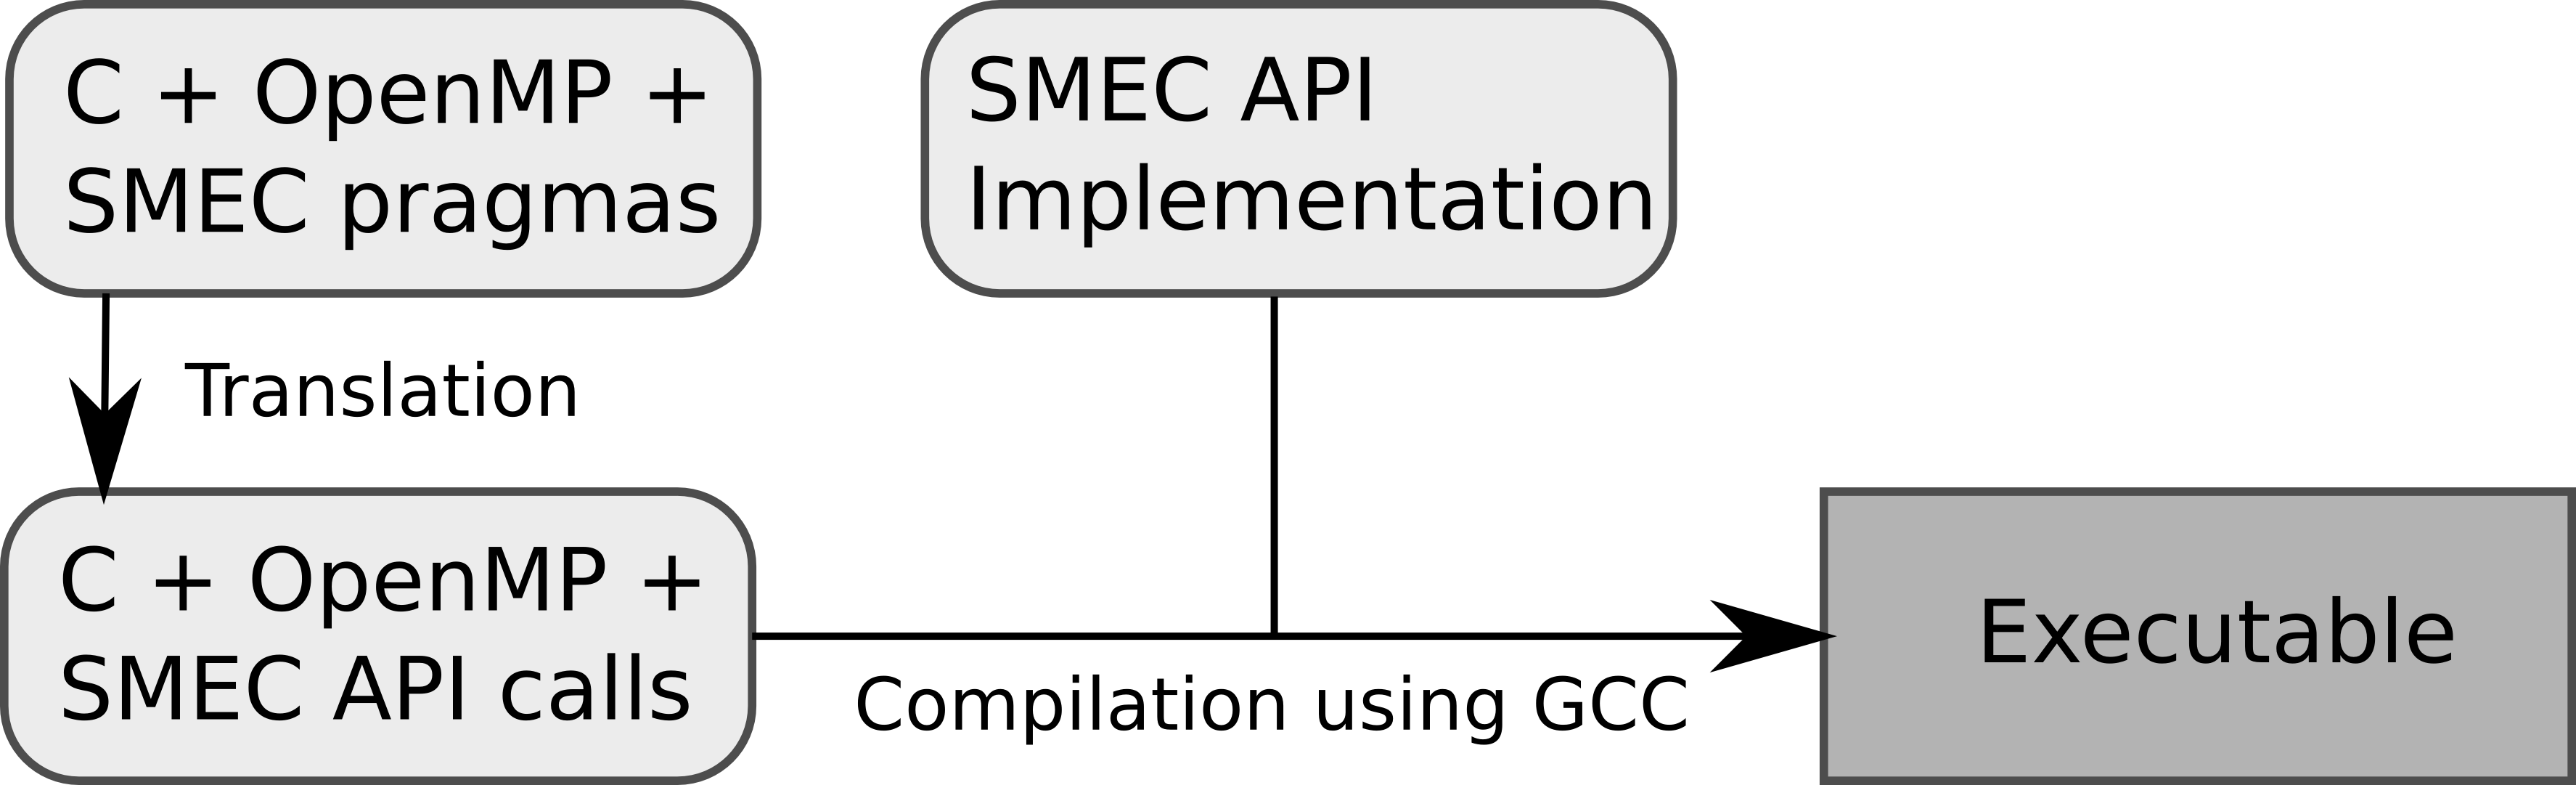
\includegraphics{compiler.png}
  \caption{Steps of the compilation of a file with SMECY pragmas and OpenMP}
\end{figure}
	
	
	\subsubsection{Mapping} Replacing the pragma and the function call with the corresponding API calls is quite straightforward with the numerous AST edition tools in ROSE. Nevertheless, some scenarios require a special handling :
	\begin{itemize}
		\item If an \verb+If+ clause is present then the API calls and
          function calls will be both kept and organized as follows:
		\begin{lstlisting}[frame=none, numbers=none]
if (condition)
	/* SMECY API calls */
else
	/* original function call */
		\end{lstlisting}
		\item If an \verb+If+ clause is present and if the function call is also a variable declaration (for example \verb+int a = f()+) then the variable declaration must be moved outside the \verb+if+ as follows:
		\begin{lstlisting}[frame=none, numbers=none]
int a;
if (condition)
	/* SMECY API calls */
	a = SMECY_get_return(/* parameters */);
else
	a = f();
		\end{lstlisting}
		\item If the pragma itself is the single-statement body of a C control 
          structure  (such as a \verb+for+ or a \verb+while+) then ROSE parser will parse it wrongly since it
          does not know that the SMECY pragma applies to the following
          function call. The function call will be the next statement
          after the structure instead of being the body of the pragma
          declaration. The following source code is an example of a case where parsing is not done well:
          \begin{lstlisting}[frame=none, numbers=none]
/* ROSE parser thinks the pragma
line is the body of the for loop*/
for (int i=0; i<10; i++)
#pragma smecy map(PE,i)
	func();
		\end{lstlisting}

		This situation requires fetching the function call, creating a multi-statement body around the pragma and moving the function call in it, right after the pragma.
	\end{itemize}
	
	Taking these special scenarios into account, the complete algorithm to transform \verb+map+ directives into SMECY API is:
	\begin{enumerate}
		\item Make sure the SMECY pragma is in a multi-statement body. If not, fetch the function call and create the multi-statement body.
		\item If the function call is a variable declaration, move the declaration itself before the pragma and make the function call a simple assignation.
		\item If there is an \verb+If(condition)+ clause put the pragma and the function calls in a C \verb+if+ structure as follows:
		\begin{lstlisting}[frame=none, numbers=none]
if (condition)
	/* the pragma declaration */
else
	/* the function call */
		\end{lstlisting}
		\item Add a \verb+SMECY_set+ before the pragma declaration
		\item For each input parameter in the function call add a \verb+SMECY_send_arg+ or \verb+SMECY_send_arg_vector+ before the pragma declaration.
		\item For each output parameter in the function call add a \verb+SMECY_get_arg_vector+ after the pragma declaration.
		\item If the function call was an assignment to variable \verb+v+ replace the pragma with \verb+v = SMECY_get_return(/* parameters */)+.
		\item If there was no \verb+If+ clause, remove the function call.
	\end{enumerate}

	\subsubsection{Streaming} Once again, ROSE provides all the necessary tools to add the pieces of code mentioned above to the original code but this time the transformation is more than replacing some code. Several delicate points must be considered:
	\begin{itemize}
		\item the definitions of the nodes' newly created functions cannot be placed anywhere since they require the newly created struct type and the function originally pointed out by the \verb+stream_node+ pragma. Consequently, they are being placed right before the definition of the function containing the original \verb+stream_loop+ directive;
        \item the declaration of the \texttt{struct} type is placed right above them.
	\end{itemize}
	
	%All these remarks have been taken into account in the following algorithm:
	%\begin{enumerate}
	%	\item
	%\end{enumerate}
	
	%FIXME expand this part
 
 	\paragraph{Using macros}
	
	The example translated source code for streaming (source code \ref{streamoutput}) is far from simple. The source code \ref{macros} below shows how
    \emph{C macros} could be used to simplify the output code and the translation process.

	\begin{lstlisting}[label=macros,caption={Streaming output code with
macro calls. The definitions of \texttt{Produce} and \texttt{Consume} functions are not shown.}]
#include "p4a_macros.h" 

struct __buffer_type_0 {
	int data_buffer;
};

void __Node_0_0() {
	__buffer_type_0* struct_buffer;
	p4a_stream_get_init_buf(0);
	while(1){
		Produce(struct_buffer -> data_buffer);
		p4a_stream_put_data(0);
	}
}

void __Node_0_1() {
	__buffer_type_0 *struct_buffer;
	while(1){
		p4a_stream_get_data(0);
		Consume(struct_buffer -> data_buffer);
	}
}

int main() {
	data_buff data_buffer ;
	p4a_init_stream(0);
	p4a_launch_stream(0,0);
	p4a_launch_stream(0,1);
	pause();
	return 0;
}
	\end{lstlisting}

	The translator built using ROSE does not need to know the \verb+P4A_+
    calls will be expanded when output code is compiled. Using such macros
    not only allows for a simpler translation and a more readable output
    code but it also encapsulates the API calls. It means the produced
    code becomes independent of the use of the SMECY API and independent
    of the way the pipeline is really implemented.
    
    \subsubsection{Mapping in conjunction with streaming}
 Practically there is not much to do to compile source codes such as source code \ref{conjin}. After the \verb+stream_loop+ has been processed a function has been created for each node. This function contains a call to the function originally pointed by the \verb+stream_node+ pragma. The compiler function that process the \verb+map+ directives just needs to be called on this function with the original \verb+stream_node+ pragma.

\section{Perspectives and conclusions}
	\subsection{Tests}
	Since SME-C is an ongoing project, no implementation of the SMECY API existed when the compiler was tested. I have written an "empty" (i.e with functions that do nothing) implementation so as to check at least the syntax of the translated source code. I have also written an example-specific OpenMP implementation to run a full test on one example.
	
	Examples were provided with the SME-C specifications. Most of them were correctly compiled. Some were impossible to compile due to the unfinished state of the specifications (remapping). One example was fully tested using a specific implementation of the SMECY API and was compiled and run correctly.
	
	\subsection{Possible improvements}
	The main limitation of the compiler prototype is the need for user-provided information. Analyses could be made to automate the gathering of information about arguments. Such analyses could be implemented using some of ROSE analysis tools like the virtual Control Flow Graphs \cite{tuto}.
	
	If such a mechanism was present, \verb+arg+ clauses would not be necessary (although they would remain useful to minimize data transfers). It means that \verb+map+ and \verb+stream_node+ directives could be applied to blocks of code instead of just function calls. This would easily be done using the ROSE outliner \cite{tuto,outliner}.
	
	\subsection{Conclusion}
	Although the SME-C compiler could not be run because of the lack of
    SMECY API implementation, the use of the ROSE compiler infrastructure
    proved successful in translating SMECY pragmas to a lower-level
    API.
    
    Breaking down the problem into several layers (pragmas, macros
    and API) and into several steps (source-to-source translation then compilation) turned out to be an efficient approach and made it possible to build a full specialized C compiler in the course of the internship.
    In the field of embedded manycore systems heterogeneous accelerators, which is all about saving time with parallelization and adapting to quickly-evolving technologies, it is impossible to write a new compiler from scratch each time a new one is needed. This internship showed that using the ROSE compiler infrastructure in conjunction with existing compilers is a very efficient way to build specialized compilers.
	
	%FIXME expand a bit
	
	\newpage
	\appendix
	\section{SMECY API}
	\label{api}
	\subsection{SMECY API}
	This is the list of the functions in the low-level SMECY API
    \cite{smec} used to control hardware accelerators in a rather portable
    way.
	\begin{lstlisting}[frame=none,numbers=none]
/* Prepare a processing element to execute a function

   @param pe is the symbol of a processing element, such as GPP, DSP, PE...
   @param[in] instance is the instance number of the processor element to use
   @param func is the function to load on the processor element
*/
#define SMECY_set(pe, instance, func) ...

/* Send a scalar argument to a function on a processing element

   @param pe is the symbol of a processing element, such as GPP, DSP, PE...
   @param[in] instance is the instance number of the processor element to use
   @param func is the function to load on the processor element
   @param[in] arg is the argument instance to set
   @param type is the type of the scalar argument to send
   @param[in] val is the value of the argument to send
*/
#define SMECY_send_arg(pe, instance, func, arg, type, val) ...

/* Send a vector argument to a function on a processing element

   @param pe is the symbol of a processing element, such as GPP, DSP, PE...
   @param[in] instance is the instance number of the processor element to use
   @param func is the function to load on the processor element
   @param[in] arg is the argument instance to set
   @param type is the type of the vector element to send
   @param[in] addr is the starting address of the vector to read from
              caller memory
   @param[in] size is the length of the vector
*/
#define SMECY_send_arg_vector(pe, instance, func, arg, type, addr, size) ...

/* Launch the hardware function or remote program using previously loaded
   arguments

   @param pe is the symbol of a processing element, such as GPP, DSP, PE...
   @param[in] instance is the instance number of the processor element to use
   @param func is the function to load on the processor element

   A kernel can be launched several times without having to set/reset
   its function.
*/
#define SMECY_launch(pe, instance, func) ...

/* Get the return value of a function on a processing element

   @param pe is the symbol of a processing element, such as GPP, DSP, PE...
   @param[in] instance is the instance number of the processor element to use
   @param func is the function to load on the processor element
   @param type is the type of the scalar argument to send
   @return the value computed by the function
*/
#define SMECY_get_return(pe, instance, func, type) ...

/* Get a vector value computed by a function on a processing element

   @param pe is the symbol of a processing element, such as GPP, DSP, PE...
   @param[in] instance is the instance number of the processor element to use
   @param func is the function to load on the processor element
   @param[in] arg is the argument instance to retrieve
   @param type is the type of the vector element
   @param[out] addr is the starting address of the vector to write in
               caller memory
   @param[in] size is the length of the vector
*/
#define SMECY_get_arg_vector(pe, instance, func, arg, type, addr, size) ...

/* Reset a processing element to execute a function

   @param pe is the symbol of a processing element, such as GPP, DSP, PE...
   @param[in] instance is the instance number of the processor element to use
   @param func is the function to unload from the processor element

   This is used for example to remove consuming resources to decrease
   power. Giving here the function name may be useful for weird case to
   avoid having short-circuit between CLB in a FPGA during unconfiguring stuff
*/
#define SMECY_reset(pe, instance, func) ...
	\end{lstlisting}
	
	\subsection{Streaming API}
	The following is not strictly part of the SMECY API \cite{smec}. It
    contains some runtime functions needed for a streaming implementation.
	\begin{lstlisting}[frame=none, numbers=none]
/*
 * Create a double buffered communication link,
 * with each buffer the given size in bytes */
DbLink createDbLink( int size ) ;
/*
 * Get a pointer to a free output buffer from the
 * link. The pointer must be given back in the
 * call to DbLinkPutData */
void *DbLinkGetInitBuf( DbLink outputLink ) ;
/*
 * Get a pointer to data out of the link. This
 * is a read action of the link. The data pointed
 * to is valid until the next read. */
void *DbLinkGetData( DbLink inputLink ) ;
/*
 * Output the data pointed to over the link. The
 * pointer must have been previously obtained from
 * the link. */
data_bufferOut = DbLinkPutData( data_bufferOut ) ;
	\end{lstlisting} 

	There is also a process creation function.
	\begin{lstlisting}[frame=none, numbers=none]
int pth_CreateProcess( int (*f)(), ... );
	\end{lstlisting}
	

	\bibliography{biblio}{}
	\bibliographystyle{plain} 

	
\end{document}

% Emacs religion:
%%% Local Variables:
%%% mode: latex
%%% ispell-local-dictionary: "american"
%%% TeX-PDF-mode: t
%%% TeX-master: t
%%% End:

% Be fair, vi religion too :-)
% vim: spell spelllang=en
